\titreTD{\thenumTD}{M\'esom\'erie}

\exo{Formes limites}

Donner la structure de Lewis et la g\'eom\'etrie de l'ion carbonate CO$_3^{2-}$. 
L'exp\'erience montre que pour cet ion les liasons C-O sont \'equivalentes (0.129~nm).
Justifier ce r\'esultat.

\exo{Effets +M et -M sur des syst\`emes simples}

En justifiant par l'hybridation des atomes ($sp$, $sp^2$, $sp^3$), identifiez les sites donneurs et 
accepteurs de m\'esom\'erie (+M et $-$M) des structures de Lewis suivantes, et proposez un sch\'ema 
envisageable de mobilit\'e \'electronique (avec 1 ou 2 fl\`eches).

\begin{center}
\begin{tabular}{ccccc}
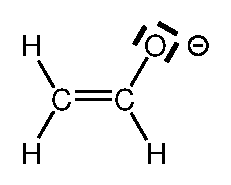
\includegraphics[scale=0.7]{figure/meso1.eps} & \, & 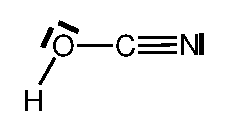
\includegraphics[scale=0.7]{figure/meso2.eps} & \, &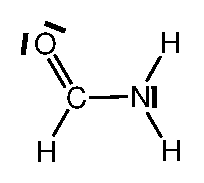
\includegraphics[scale=0.7]{figure/meso3.eps} \\
1& &2& &3\\[0.2cm]
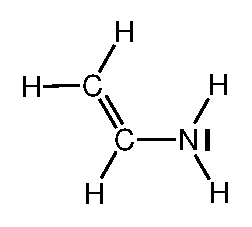
\includegraphics[scale=0.7]{figure/meso4.eps} &    &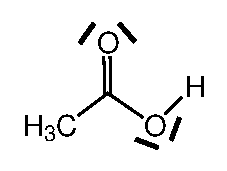
\includegraphics[scale=0.7]{figure/meso5.eps} &  &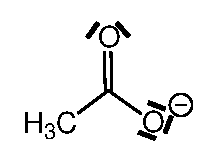
\includegraphics[scale=0.7]{figure/meso6.eps} \\
4& &5&  &6\\
\end{tabular}
\end{center}

\exo{Cas r\'eels}
\'Etablir la structure de Lewis des mol\'ecules suivantes, et donnez leurs formes m\'esom\`eres 
les plus probables selon les r\`egles usuelles (respect de l'octet, limitation de la s\'eparation de charge, etc...).

%\begin{figure}[!h]
\begin{center}
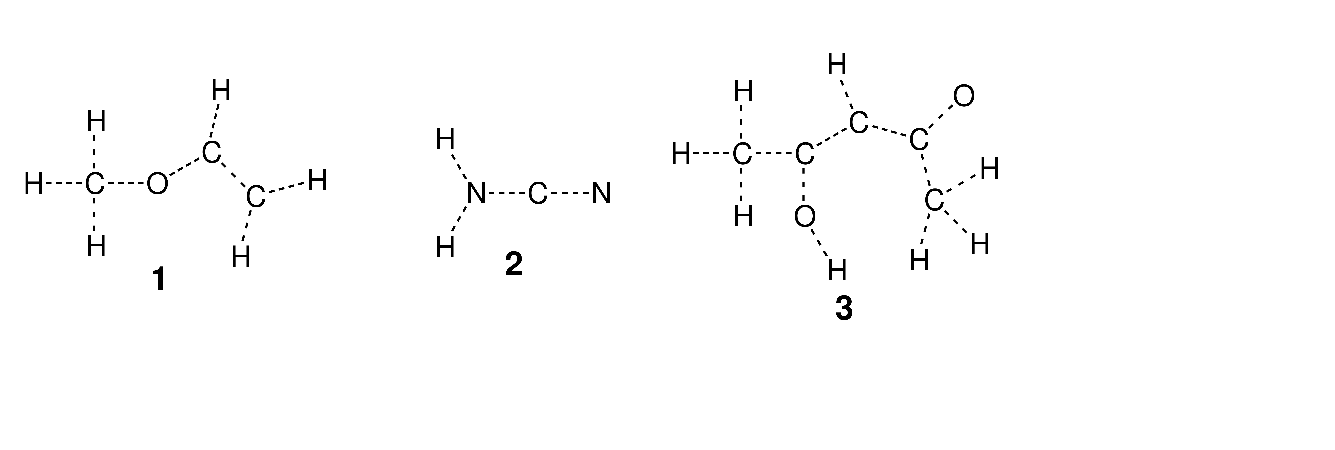
\includegraphics[scale=0.77]{figure/lewis4.eps}
\end{center}
%\end{figure}

\vrule

\clearpage

\exo{M\'esom\'erie}

Proposez un sch\'ema envisageable de mobilit\'e \'electronique (avec 1 ou 2 fl\`eches) pour
les mol\'ecules suivantes~:

\begin{center}
\begin{tabular}{ccc}
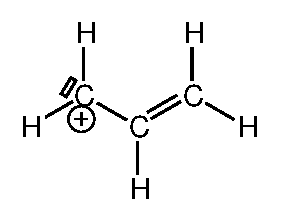
\includegraphics[scale=0.7]{figure/ex2meso1.eps} & \, & 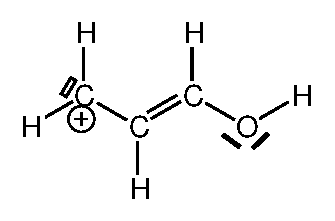
\includegraphics[scale=0.7]{figure/ex2meso2.eps} \\
1&&2\\[0.2cm]
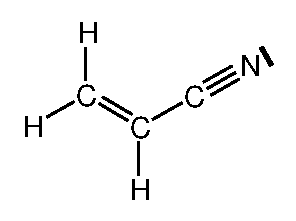
\includegraphics[scale=0.7]{figure/ex2meso3.eps} & \, & 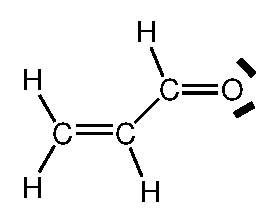
\includegraphics[scale=0.7]{figure/acrolein.eps} \\
3&&4\\
\end{tabular}
\end{center}



